\chapter{Experiments}
\label{cha:experiments}
\vspace{0.4 cm}

In this chapter, we're going to delve into the experiments we've crafted to put our approach into action and assess its performance. We'll walk you through the design, implementation, and evaluation steps, providing a detailed account of each experiment. These experiments are crucial to demonstrating the effectiveness and practicality of our approach in real-world scenarios. The source code for our implementation of the tool can be found in the added references~\cite{evooracle_github}\cite{evooracle_gitlab}.

\section{Data Collection}
\label{sec:data_collection}
\vspace{0.2 cm}
Within this sub-chapter, we will elaborate on our methodology for assembling a collection of Java projects. We outline the procedures involved in generating test cases using automated tools such as EvoSuite and Randoop\cite{noauthor_randoop_nodate}, shedding light on the meticulous steps taken to ensure comprehensive test coverage. Additionally, we will discuss the meticulous process of preparing corresponding focal methods, elucidating how we identify and associate the specific methods targeted by each test case. This step is crucial in establishing a robust foundation for subsequent analyses and evaluations within the realm of software testing and development.

\vspace{0.1 cm}
\subsection{Java Projects Selection}
\label{sec:projects_selection}
\vspace{0.1 cm}

We carefully selected four projects, as outlined in Table \ref{tab:collected_java_projects}, from the pool of publicly available GitHub Java repositories that declare an open-source license. Our selection criteria also considered popularity, with priority given to projects boasting the highest number of stars or forks. Emphasizing diversity, we aimed to cover a spectrum of project types. Here are the project selection criteria that we followed:\\
    \begin{enumerate}
        \item \textbf{Preventing Data Leakage:} To mitigate the risk of unintentional data exposure, we systematically exclude potential repositories that might be part of the pretraining data for the considered Large Language Models (LLMs). Our focus lies on projects updated within the past three years to ensure relevance.
        
        \item \textbf{Maven Compatibility:} To streamline subsequent processes, we narrow down our dataset to repositories utilizing Maven as the package manager. This decision is based on the presence of a pom.xml file at the repository root, indicating Maven usage.

        \item \textbf{Class Threshold:} We eliminate repositories with fewer than 40 classes to avoid selecting overly simplistic projects that might not offer substantial complexity.
        
        \item \textbf{Compilation Check:} Ensuring the compilability of repositories is crucial. We mandate that all dependencies be specified in the pom.xml files and selected Java version (Java 1.8). The compilation process is executed with the command 
        \begin{verbatim}
        mvn clean compile
        \end{verbatim} and repositories failing to compile are excluded. Although roughly half of the repositories compile successfully, further exploration of compilation errors might enhance compilation success rates in future endeavors.
        
        \item \textbf{Execution Check:} Similar to the compilation criterion, we require repositories to be executable in our environment. Following the selection of the Java version, we execute the command 
        \begin{verbatim}
        cd target
        java -jar <PROJECT-SNAPSHOT>.jar
        \end{verbatim}
        and retain repositories where the command succeeds. Logs are saved for future reference, and potential investigation into reasons for execution failures is left for future work.
    \end{enumerate}
From these chosen projects, encompassing a total of 388 classes, we further refined our sample by randomly selecting nine classes, totaling 87 methods. This thoughtful selection process ensures that our tool encounters a diverse range of scenarios and project structures, contributing to a more comprehensive evaluation. Further details about these chosen classes can be found in Table \ref{tab:selected_java_projects}.

\begin{table}[htbp]
    \centering
    \begin{tabular}{l | l | r}
        \textbf{Project Name} & \textbf{Classes} & \textbf{Reference} \\
        \hline
        frontend-maven-plugin & 43 & \cite{sletteberg_frontend-maven-plugin_2023} \\
        javacv & 117 & \cite{noauthor_bytedecojavacv_nodate} \\
        webdrivermanager & 44 & \cite{noauthor_bonigarciawebdrivermanager_nodate} \\
        zerocode & 184 & \cite{noauthor_authorjappszerocode_nodate} \\
    \end{tabular}
\caption{Details of the collected Java projects.}
\label{tab:collected_java_projects}
\end{table}

\begin{table}
    \centering    
    \begin{tabular}{l | l | r}
        \textbf{Class Name} & \textbf{Project Name} & \textbf{Methods} \\
        \hline
        BaseSettings & javacv & 6 \\
        Parallel & javacv & 6 \\
        SeekableByteArrayOutputStream & javacv & 3 \\
        NPMInstaller & frontend-maven-plugin & 15 \\
        NodeInstaller & frontend-maven-plugin & 18 \\
        PnpmInstaller & frontend-maven-plugin & 14 \\
        CacheHandler & webdrivermanager & 4 \\
        PropertiesProviderUtils & zerocode & 4 \\
        ZerocodeCorrelationshipLogger & zerocode & 17 \\
    \end{tabular}
\caption{Details of the classes from the selected Java projects.}
\label{tab:selected_java_projects}
\end{table}

\vspace{0.1 cm}
\subsection{Test Case Generation with EvoSuite}
\label{sec:test_case_generation}
\vspace{0.1 cm}

Our tool is designed to enhance existing test cases by focusing on improving assertions. To achieve this, we require one or more test suites, and for our research, we've opted to use EvoSuite. EvoSuite\cite{noauthor_evosuite_nodate} is a sophisticated tool specifically tailored for automatically generating test cases with assertions for Java code. It employs a unique hybrid approach that not only generates but also optimizes entire test suites to fulfill specific coverage criteria. These criteria guide the tool in producing comprehensive test suites that effectively cover the targeted code. EvoSuite doesn't stop at merely generating tests; it goes a step further by suggesting potential oracles for these test cases. Oracles, in this context, are sets of assertions strategically added to succinctly summarize the current behavior of the code. These assertions serve a crucial role—enabling developers to identify deviations from expected behavior and capturing the existing behavior to safeguard against potential defects in the future.

For our study, we utilized EvoSuite to generate automated test cases for each of the selected classes. We adhered to the default configurations of EvoSuite, setting the search budget to 15 and opting not to minimize. We generated 9 Test Suites with a total of 138 test cases. The generated test suites for each class are outlined in Table \ref{tab:evosuite_testclasses}.

\begin{table}
    \centering    
    \begin{tabular}{l | l | r}
        \textbf{Test Suite} & \textbf{Class Name} & \textbf{Test Cases} \\
        \hline
        BaseSettings\_ESTest & BaseSettings & 14 \\
        Parallel\_ESTest & Parallel & 6 \\
        SeekableByteArrayOutputStream\_ESTest & SeekableByteArrayOutputStream & 13 \\
        NPMInstaller\_ESTest & NPMInstaller & 18 \\
        NodeInstaller\_ESTest & NodeInstaller & 18 \\
        PnpmInstaller\_ESTest & PnpmInstaller & 21 \\
        CacheHandler\_ESTest & CacheHandler & 13 \\
        PropertiesProviderUtils\_ESTest & PropertiesProviderUtils & 14 \\
        ZerocodeCorrelationshipLogger\_ESTest & ZerocodeCorrelationshipLogger & 21 \\
    \end{tabular}
\caption{Summary of EvoSuite generated test classes.}
\label{tab:evosuite_testclasses}
\end{table}

\vspace{0.1 cm}
\subsection{Metadata Extraction}
\label{sec:data_extraction}
\vspace{0.1 cm}

This step involves parsing each project to extract essential information about classes and methods, along with their associated metadata. Once this information is obtained, our focus shifts to identifying test classes and establishing their connections with corresponding focal classes. This pivotal step ensures that we precisely match each test class with its relevant counterpart. Following the identification of test classes and their associations, we move on to a crucial mapping process. For every test case within a test class, we meticulously map it to the corresponding focal method. This meticulous mapping results in a comprehensive set of mapped test cases, forming the foundation for subsequent stages in our methodology.

\begin{itemize}
  \item \textbf{Parsing:} In the parsing phase, we thoroughly analyze each project using the tree-sitter parser\cite{noauthor_tree-sitterintroduction_nodate}. This process involves extracting valuable metadata linked to the identified classes and methods within the project. The collected information encompasses crucial details like class names, signatures, super class, bodies, annotations, interfaces, package, imports, fields, arguments list, constructors, dependencies and variables, method names, return types, any developer written comments. This parsed code serves a dual purpose: firstly, to pinpoint test cases and their corresponding focal methods, and secondly, to enhance the focal methods by incorporating focal context information.
                                
  \item \textbf{Identify Test Classes:} In this stage, our goal is to locate all the test classes within the project. Test classes are those classes housing at least one method annotated with the \textit{\textbf{@Test}} annotation. This specific annotation serves as an indicator to JUnit, signaling that the attached method is eligible to be executed as a test case. By identifying and marking classes in this manner, we establish a clear distinction between regular classes and those instrumental to the testing process. This categorization allows a systematic approach to handling test-related components.

  \item \textbf{Identify Focal Classes:} Identifying Focal Classes involves determining the class under test for each test class. We employ a two-step approach using the following heuristics:
        \begin{enumerate}
            \item \textbf{Extracting Class Instances:} The initial heuristic involves analyzing each test method to identify all the classes instantiated or any objects created during the testing process.
            \item \textbf{Matching Class Names:} Subsequently, we employ name matching as the second heuristic. Test classes typically follow a naming convention that includes the name of the focal class, often with a \textit{"Test"} prefix or suffix. For instance, a test class associated with the \textit{"BaseSettings.java"} class might be named \textit{"BaseSettingsTest.java"} or, in the case of Evosuite, \textit{"BaseSettings\_ESTest.java."} To identify the focal class, we perform name matching by comparing the name of the test class (minus the optional \textit{"\_ESTest"} suffix) with potential focal classes. This step ensures a robust association between test classes and their corresponding focal classes.
        \end{enumerate}

  \item \textbf{Identify Focal Method:} Determining the focal method for each test case involves employing specific heuristics. 
  \begin{enumerate}
      \item \textbf{Matching Method Names:} This heuristic leverages the common practice of naming test cases similarly to their corresponding focal methods. This involves matching test case names with focal methods, considering potential prefixes or suffixes like "Test."
      \item \textbf{Analyzing Method Invocations:} Additionally, this heuristic is applied if the initial method doesn't identify a focal method. We try to match the last method invocation before (or within) the assert statement within the test case and the methods defined in the focal class. If a match is found, it is selected as the focal method. We also collect other method invocations as it might be useful to prepare the focal context. This approach is grounded in the confidence gained from prior matching of the test class to the focal class, making it likely that the test case is specifically targeting that single method.
  \end{enumerate}

  Following these heuristics, we obtain a set of test cases paired with their corresponding focal class and focal methods. Test cases where we couldn't identify the focal method using our heuristics are excluded from further consideration.
  
\end{itemize}

\section{Preprocessing}
\label{sec:preprocessing}
\vspace{0.2 cm}

The EvoOracle's prompt processor component employs a two-step approach using specific heuristics to preprocess test cases, ensuring they are appropriately prepared for prompt generation. We used the regex pattern shown in Listing~\ref{assertions_regex} for both the following steps:

    \begin{enumerate}
        \item \textbf{Removal of Assertions:} All selected test cases undergo the removal of assertions, retaining only the last assertion in case there are multiple assertions using Algorithm~\ref{algorithm_remove_assertion}. This decision is based on the likelihood that reaching the last assertion implies satisfaction of all preceding assertions. This is a reasonable choice which is also seen in the work of Tufano et al. \cite{tufano_generating_2022}. The purpose is to streamline the test cases for further processing.

        \item \textbf{Placeholder Insertion:} Following the removal of additional assertions, the test cases are left with a single assertion. We replace this single assertion with \textit{"\_\_ASSERTION\_PLACEHOLDER\_\_"} placeholder using Algorithm~\ref{algorithm_placeholder_insertion}. This placeholder serves as a temporary marker and will be subsequently replaced with assertions generated by the Large Language Models.
    \end{enumerate}

    %Assertion selection Regex highlighting
    \hrule
    \begin{lstlisting}[language=Python, caption=Assertion selection Regex, label=assertions_regex]
    assertion_patterns = [
        r'(\w+\.)?assert\s*\(.+?\);',           # ClassName.assert(...)
        r'(\w+\.)?assertTrue\s*\(.+?\);',       # ClassName.assertTrue(...)
        r'(\w+\.)?assertNull\s*\(.+?\);',       # ClassName.assertNull(...)
        r'(\w+\.)?fail\s*\(.+?\);',             # ClassName.fail(...)
        r'(\w+\.)?assertFalse\s*\(.+?\);',      # ClassName.assertFalse(...)
        r'(\w+\.)?assertNotEquals\s*\(.+?\);',  # ClassName.assertNotEquals(...)
        r'(\w+\.)?assertEquals\s*\(.+?\);',     # ClassName.assertEquals(...)
        r'(\w+\.)?assertArrayEquals\s*\(.+?\);',# ClassName.assertArrayEquals(...)
        r'(\w+\.)?assertNotNull\s*\(.+?\);',    # ClassName.assertNotNull(...)
        r'(\w+\.)?assertNotSame\s*\(.+?\);',    # ClassName.assertNotSame(...)
        r'(\w+\.)?assertSame\s*\(.+?\);',       # ClassName.assertSame(...)
        r'(\w+\.)?assertThat\s*\(.+?\);',       # ClassName.assertThat(...)
    ]
    \end{lstlisting}
    \hrule
    
    \begin{algorithm}[H]
    \caption{Algorithm for \texttt{Removing all assertions but last}}
    \label{algorithm_remove_assertion}
    \begin{algorithmic}[1]
    \Function{remove\_all\_assertions\_but\_last}{$\text{source\_code}$}
        \State $\text{assertion\_patterns} \gets$ [\texttt{...}] \Comment{List of assertion patterns}
        \State $\text{assertions} \gets \text{re.findall(assertion\_pattern, source\_code)}$
    
        \If{\text{not assertions}}
            \State \textbf{return} $\text{source\_code}$
        \EndIf
    
        \State $\text{replaced\_assertions} \gets []$
    
        \For{$i$ \textbf{in} \text{range}(\text{len(assertions) - 1})}
            \State $\text{source\_code} \gets \text{re.sub(assertion\_pattern, "", source\_code, count=1)}$
            % \State $\text{replaced\_assertions.append(assertions[i][0] + assertions[i][1] + "();")}$  % Uncomment this line if you want to keep track of removed assertions
        \EndFor
    
        \State \textbf{return} $\text{source\_code}$
    \EndFunction
    \end{algorithmic}
    \end{algorithm}

    \begin{algorithm}
    \caption{Algorithm for \texttt{Placeholder insertion}}
    \label{algorithm_placeholder_insertion}
    \begin{algorithmic}[1]
    \Function{replace\_assertions}{$\text{source\_code}$}
        \State $\text{assertion\_patterns} \gets$ [\texttt{...}] \Comment{List of assertion patterns}
        \State $\text{replaced\_assertions} \gets$ [] \Comment{List to store replaced assertions}
    
        \For{$\text{pattern}$ \textbf{in} $\text{assertion\_patterns}$}
            \Function{replacement}{$\text{match}$}
                \State $\text{matched\_text} \gets \text{match.group(0)}$
                \State $\text{replaced\_assertions.append(matched\_text)}$
                \State \textbf{return} \texttt{(ASSERTION\_PLACEHOLDER)}
            \EndFunction
    
            \State $\text{source\_code} \gets \text{re.sub(pattern, replacement, source\_code)}$
        \EndFor
    
        \State \textbf{return} $\text{source\_code, replaced\_assertions}$
    \EndFunction
    \end{algorithmic}
    \end{algorithm}
        
\section{Large Language Model Integration}
\label{sec:llm_integration}
\vspace{0.2 cm}

To improve the Oracles generated by the automated test generation tools, we propose the inclusion of LLMs into the test generation process. Recognizing that LLMs typically demand substantial resources and powerful hardware, we opted to leverage GPT4All~\cite{noauthor_gpt4all_nodate} to make this solution accessible to developers on standard development machines.

\textbf{GPT4All:} The GPT4All~\cite{noauthor_gpt4all_nodate} project, initiated by Nomic AI, seeks to democratize access to Large Language Models by enabling training and deployment on common hardware. This open-source ecosystem facilitates the integration of LLMs into applications without the need for costly platform subscriptions or specialized hardware. Notably, GPT4All addresses accessibility by providing pretrained models with reduced sizes, ensuring they can operate efficiently on CPUs, even on PCs lacking internet connectivity or a GPU. This innovation allows smaller entities and independent researchers to harness LLMs for various applications, such as content creation, coding, document comprehension, and information retrieval. With a user-friendly one-click installer, GPT4All streamlines the process, making LLM utilization feasible on modern PCs with 4–16GB of RAM, a substantial reduction compared to traditional requirements, thanks to neural network quantization~\cite{han_deep_2016}.

\vspace{0.1 cm}
\subsection{LLM Selection and Configuration}
\label{sec:llm_configurations}
\vspace{0.1 cm}

Our tool offers flexibility in LLM selection, allowing developers to choose models based on their preferences. To seamlessly integrate a specific LLM into our framework, developers need to load the corresponding configurations for that particular model. For our experiments, we opted for models acknowledged for their performance, relying on the HuggingFace\cite{noauthor_hugging_2023} Open LLM Leaderboard\cite{open-llm-leaderboard} as a reference. We carefully selected five top-performing models, as highlighted in Table~\ref{tab:selected_models}, presenting the LLM benchmark.

This approach empowers users to tailor their LLM choices, ensuring compatibility and aligning with their project requirements. The decision to incorporate well-regarded models from the leaderboard enhances the credibility and effectiveness of our experiments.

\begin{table}[htbp]
    \centering    
    \begin{tabular}{l | c | c | c | c | c | r}
        \textbf{Model} & \textbf{Average} & \textbf{ARC} & \textbf{HellaSwag} & \textbf{MMLU} & \textbf{TruthfulQA} & \textbf{Reference} \\
        \hline
        \scriptsize\textsc{mpt-7b-chat} & 49.95 & 46.5 & 75.51 & 37.62 & 40.16 & \cite{MosaicML2023Introducing}\cite{noauthor_mosaicmlmpt-7b-chat_2023}  \\
        \scriptsize\textsc{Nous-Hermes-13b} & 60.15 & 56.57 & 82.11 & 50.44 & 51.5 & \cite{noauthor_nousresearchnous-hermes-13b_nodate} \\
        \scriptsize\textsc{orca\_mini\_v3\_13b}  & \textbf{63.45*} & \textbf{63.14*} & \textbf{82.35*} & \textbf{56.52*} & 51.81 & \cite{noauthor_pankajmathurorca_mini_v3_13b_2023}\cite{mukherjee2023orca}\\
        \scriptsize\textsc{stable-vicuna-13B}  & 57.63 & 53.33 & 78.5 & 50.29 & 48.38 & \cite{noauthor_theblokestable-vicuna-13b-hf_2023} \\
        \scriptsize\textsc{WizardLM-13B-V1.1}  & 60.55 & 58.62 & 81.07 & 48.32 & \textbf{54.19*} & \cite{noauthor_theblokewizardlm-13b-v1-1-superhot-8k-fp16_nodate}\cite{vicuna2023} \\
    \end{tabular}
\caption{OpenLLM Leaderboard Benchmarks for Selected Models}
\label{tab:selected_models}
\end{table}

In the preliminary phase of our experimentation, we conducted local trials with various configurations to fine-tune the settings for our Large Language Models (LLMs). These configurations play a pivotal role in shaping the characteristics of our tool, EvoOracle, which focuses on test oracle generation. Based on the results obtained from our local experiments and considering the significance of each configuration parameter, we opted for a set of parameters that strike a delicate balance between precision, diversity, and computational efficiency. With a low temperature of 0.1, our chosen configuration ensures deterministic and focused predictions. Simultaneously, the generous n\_predict value of 4096 allows for a broad spectrum of predictions, promoting diversity. Setting top-p to 0.95 and top-k to 40 emphasizes the consideration of high-probability tokens during sampling. The chosen batch size of 9 optimizes computational resources. Lastly, the repeat penalty and repeat last N parameters, both set at 1.1, encourage non-repetitive and varied output. This meticulous selection of configurations from our local trials serves as a foundation for the subsequent large-scale experiments on the cluster, ensuring an optimal balance between assertive precision and computational efficiency.

\vspace{0.1 cm}
\subsection{Prompt Preparation}
\label{sec:prompt_preparation}
\vspace{0.1 cm}

In the critical phase of prompting the Large Language Models for assertion generation, we employ a meticulous approach. To facilitate this process, we construct prompt templates using the versatile Jinja2\cite{noauthor_jinja_nodate}
template format. The essence lies in creating a focal context tailored for each Class Under Test (CUT) and its corresponding Method Under Test (MUT). These templates serve as the foundation for replacing the contextual placeholders with the specific contexts of interest. This dynamic approach ensures that the LLMs receive targeted and meaningful prompts, enhancing their understanding of the given code context and enabling them to generate assertions with precision. The use of Jinja2 templates not only streamlines the prompt generation process but also allows for flexibility and adaptability in accommodating diverse code structures across different classes and methods.

Before settling on our final approach for effective assertion generation, we conducted a series of preliminary experiments. The goal was to refine our prompt strategy, ensuring that it aligns optimally with the intricacies of the code context. After careful consideration and evaluation, we arrived at a well-crafted prompt, which is detailed in Listing~\ref{prompt_template}. This strategic decision to leverage a specific prompt stems from the insights gained through experimentation, aiming to enhance the clarity and relevance of instructions provided to the Large Language Models (LLMs). Our iterative process of refining prompts has been instrumental in shaping an approach that maximizes the LLMs' understanding of code contexts and subsequently improves the precision of assertion generation.

\begin{lstlisting}[style=llm_prompt, label=prompt_template, caption=Prompt Template]
### Instruction:
You are working with a Java project which includes a class called 
`{{ class_name }}` and has some methods.
Method details as JSON: `{{ method_details }}`.
You are tasked with generating a test oracle for a JUnit test case 
based on the above information of the method to test its functionality .
### Prompt:
In the following the test case, replace the `{{ assertion_placeholder }}` 
with one or more appropriate assertions:
```
{{ test_method_code }}
```
Write the assertion statement using following pattern:
```r'(\w+\.)?(assert|assertTrue|assertNull|fail|assertFalse|assertNotEquals
|assertEquals|assertArrayEquals|assertNotNull|assertNotSame|assertSame
|assertThat)\s*\(.+?\);'```
Assertion must end with ```;```

### Response:
\end{lstlisting}

To create effective prompts for the Large Language Models, we gather information to build the context for a test case that we prepared in the preprocessing phase (as detailed in Section~\ref{sec:preprocessing}). This information includes key details about the class under test, methods under test, and various method attributes such as Constructor signature, Class Signature, parameters, Invoked Method Signature, dependencies, return type, developer comments, source code for the test case, package, imports, Fields, and getter/setter signature. We carefully consider all invoked methods and dependencies encapsulated within the test case. In instances where the LLM response faces challenges such as token limit exceeds, we dynamically adjust the context size.

We follow an iterative process as shown in Algorithm~\ref{algorithm_prompt_generation} of generating prompts for the LLM, involving multiple rounds. Each round refines the prompt based on the LLM's response and aims to address potential challenges like token limit exceedance. The trimming process, controlled by conditional statements, adjusts the size of critical elements such as method details and test method code. This adaptive approach ensures that the prompt remains concise while retaining essential contextual information. The code systematically handles different trimming scenarios in each round, progressively refining the prompt to strike a balance between informativeness and LLM response feasibility. The overall mechanism involves generating messages from prompt templates, seeking LLM responses, and dynamically adjusting the prompt for subsequent iterations, all of which contribute to an effective and tailored interaction with the LLM.

\begin{algorithm}
    \caption{Prompt Generation Algorithm}
    \label{algorithm_prompt_generation}
    \begin{algorithmic}[1]
        \Function{generate\_prompt}{$\text{context}$}
            \State $\text{rounds}, \text{max\_attempts}, \text{prompt\_template} \gets 0, 3, \text{...}$
            \State $\text{prompts\_and\_responses} \gets []$
            
            \While{$\text{rounds} < \text{max\_attempts}$}
                \State $\text{steps}, \text{rounds} \gets 0, \text{rounds} + 1$
                \If{$\text{rounds} > 2$}
                    \State $\text{trimmed\_context} \gets \text{trim\_context(context, 3)}$
                \EndIf
                
                \If{$\text{rounds} > 1$}
                    \State $\text{trimmed\_context} \gets \text{trim\_context(context, 5)}$
                \EndIf
                
                \State $\text{messages} \gets \text{generate\_messages(prompt\_template, trimmed\_context)}$
                
                \State $\text{llm\_result} \gets \text{ask\_openLLM(messages)}$
                \State $\text{prompts\_and\_responses.append(\{"prompt": messages, "response": llm\_result\})}$
                
                \State $\text{source\_code, replaced\_assertions} \gets \text{replace\_assertions(source\_code)}$
                
                \If{$\text{assertions}$}
                    \State $\text{context} \gets \text{update\_prompt\_and\_ask\_again(context)}$
                \EndIf
            \EndWhile
            
            \State $\text{print\_and\_save\_results(prompts\_and\_responses)}$
        \EndFunction
    \end{algorithmic}
\end{algorithm}

Throughout each iteration, we analyze LLM responses to capture assertions using the specified Assertion regex, as outlined in Listing~\ref{assertions_regex}. When the parsing operation successfully identifies an assertion, we advance to the subsequent phase of crafting the test case with EvoOracle assertion. In cases where the assertion parsing is unsuccessful, we continue the iteration process until we reach the budget limit specified in the configuration. 

\section{Test Case Preparation}
\label{sec:test_case_preparation}
\vspace{0.2 cm}

In this section, ...

\vspace{0.1 cm}
\subsection{Assertion Integration}
\label{sec:assertion_integration}
\vspace{0.1 cm}

In this subsection, ...

\vspace{0.1 cm}
\subsection{Test Case Compilation}
\label{sec:test_compilation}
\vspace{0.1 cm}

In this subsection, an overview of ...

\vspace{0.1 cm}
\subsection{Test Case Execution}
\label{sec:test_execution}
\vspace{0.1 cm}

In this subsection, an overview of ...

\vspace{0.1 cm}
\subsection{Mutation Testing Execution}
\label{sec:mutation_testing_execution}
\vspace{0.1 cm}

To evaluate the generated tests, we use PIT\cite{noauthor_pit_nodate}. PIT is a mutation testing tool that evaluates the robustness of a test suite by introducing mutations (faults) into the source code and assessing whether the tests can detect these mutations.

\vspace{0.1 cm}
\subsection{Report Parsing}
\label{sec:report_parsing}
\vspace{0.1 cm}

When we execute mvn pit test, it triggers the generation of Mutation Coverage reports as artifacts. These reports provide valuable insights into the effectiveness of our test suite. To extract meaningful information, we begin by parsing the HTML reports generated by PIT. By parsing the HTML reports, we extract detailed information on line coverage, mutation coverage, and test strength for all tests associated with a particular class. This information is essential for evaluating the thoroughness and fault-detection capability of our test suite.

\section{Experimental Setup}
\label{sec:experimental_setup}
\vspace{0.2 cm}

For our experimental setup, we conducted the experiments on a dedicated High-Performance Computing (HPC) cluster equipped with four nodes. Each node features Intel Xeon CPU 6226R\cite{noauthor_intel_nodate} processors running at 2.9GHz, with a configuration of 32 CPUs and 16GB of RAM. To ensure consistency and reproducibility, we created a specialized Singularity\cite{noauthor_introduction_nodate} image tailored for our implemented tool, enabling seamless execution on the HPC cluster. This configuration allowed us to leverage the cluster's computational capabilities effectively for our experimentation.

The number of experiments is given by the equation:
\[
N_e = TC \times M \times OT \times R
\]
\noindent
Here, \\
N_e = Number of experiments\\
TC = Test Cases\\
M = Models\\
OT = Oracle Type\\
R = Repetitions\\

\vspace{0.1 cm}
\subsection{Evaluation Metrics}
\label{sec:evaluation_metrics}
\vspace{0.1 cm}

    \begin{enumerate}
        \item \textbf{Coverage Metrics:}
        \begin{itemize}
            \item \textbf{Line Coverage:} This metric measures the proportion of lines of code that are executed by the test suite. It gives an overview of how much of the code is exercised during testing.
            \item \textbf{Mutation Coverage:} PIT introduces mutations into the code and analyzes how many of these mutations are detected by the test suite. Mutation coverage reflects the ability of tests to identify and handle different types of faults.
            \item \textbf{Test Strength:} This is a comprehensive metric that considers both line coverage and mutation coverage. It provides a holistic view of how well the tests exercise the code and how effective they are at detecting mutations.
        \end{itemize}
    \end{enumerate}

    In addition to coverage, we present five count metrics to quantify the number of test cases at specific stages of the pipeline:

    \begin{enumerate}
        \item \textbf{Unique:} Count of test cases after removing duplicates.
        \item \textbf{Parsable:} Count of test cases adhering to the Java grammar, measured both absolutely and relative to the Unique count.
        \item \textbf{Compilable:} Count of test cases that successfully compiled in their scaffolding without errors, measured both absolutely and relative to the Unique count.
        \item \textbf{Executable:} Count of test cases that were executed without errors, measured both absolutely and relative to the Unique count.
        \item \textbf{Correct:} Count of test cases that were executed without errors and invoked the correct Method Under Test (MUT), measured both absolutely and relative to the Unique count. 
    \end{enumerate}
    This metric is adopted from Tufano et al. \cite{tufano_unit_2021} and provides direct comparability, despite being computed on different repositories.

\section{Research Questions}
\label{sec:research_questions}
\vspace{0.2 cm}

In this section, we will discuss the research questions which are as follows:
\begin{itemize}
    \item RQ1: How does the performance of LLM-generated assertions compare to assertions generated by traditional automated test generation tools, such as EvoSuite?

    \item RQ2: To what extent can LLMs generalize across different software projects and programming paradigms when generating test assertions?
    
    \item RQ3: To what extent is the proposed LLM-based assertion generation approach suitable for real-world software development workflows? What are the challenges and practical considerations?
\end{itemize}

\section{Results}
\label{sec:results}
\vspace{0.2 cm}

In this section, a brief introduction to ... 

\vspace{0.1 cm}
\subsection{RQ1}
\label{sec:results_rq1}
\vspace{0.1 cm}

In this subsection, an overview of ...




\begin{table}[H]
\centering

\begin{tabular}{| l | r | r | r | r | r | r |}
\hline
\multirow{2}{*}{\textbf{Class}} & \multirow{2}{*}{\textbf{EvoSuite}} & \multicolumn{5}{c|}{\textbf{EvoOracle}} \\ % Fix multicolumn formatting
\cline{3-7} % Add a horizontal line between the headers
 &  & \textbf{MPT-7B} & \textbf{Nous} & \textbf{Orca} & \textbf{Stable} & \textbf{WizardLM} \\
 &  &  & \textbf{hermes-13b} & \textbf{mini\_13B} & \textbf{Vicuna-13B} & \textbf{13B-V1.1} \\
\hline
\scriptsize\textsc{} &  &  &  &  &  &  \\
\scriptsize\textsc{BaseSettings} & 100\% & 92.75\% & 98.55\% & 85.51\% & 0\% & 21.74\% \\
\hline
\scriptsize\textsc{} &  &  &  &  &  &  \\
\scriptsize\textsc{CacheHandler} & 51.52\% & 0\% & 45.45\% & 38.38\% & 0\% & 24.24\% \\
\hline
\scriptsize\textsc{} &  &  &  &  &  &  \\
\scriptsize\textsc{NPMInstaller} & 46.49\% & 6.14\% & 19.3\% & 2.05\% & 6.14\% & 6.14\% \\
\hline
\scriptsize\textsc{} &  &  &  &  &  &  \\
\scriptsize\textsc{NodeInstaller} & 53.04\% & 25.97\% & 40.51\% & 14.18\% & 0\% & 11.97\% \\
\hline
\scriptsize\textsc{} &  &  &  &  &  &  \\
\scriptsize\textsc{Parallel} & 100\% & 21.14\% & 94.31\% & 0\% & 82.93\% & 86.18\% \\
\hline
\scriptsize\textsc{} &  &  &  &  &  &  \\
\scriptsize\textsc{PnpmInstaller} & 41.53\% & 19.21\% & 25.99\% & 11.02\% & 3.67\% & 10.17\% \\
\hline
\scriptsize\textsc{Properties} &  &  &  &  &  &  \\
\scriptsize\textsc{ProviderUtils} & 57.14\% & 38.09\% & 40.47\% & 25\% & 0\% & 47.62\% \\
\hline
\scriptsize\textsc{} &  &  &  &  &  &  \\
\scriptsize\textsc{ResolutionCache} & 18.92\% & 18.92\% & 18.92\% & 6.31\% & 18.92\% & 18.92\% \\
\hline
\scriptsize\textsc{SeekableByte} &  &  &  &  &  &  \\
\scriptsize\textsc{ArrayOutputStream} & 100\% & 12.5\% & 66.67\% & 18.75\% & 31.25\% & 43.75\% \\
\hline
\scriptsize\textsc{Zerocode} &  &  &  &  &  &  \\
\scriptsize\textsc{Correlationship} &  &  &  &  &  &  \\
\scriptsize\textsc{Logger} & 91.38\% & 36.21\% & 83.91\% & 1.15\% & 0\% & 52.87\% \\
\hline

\end{tabular}
\caption{Average Line Coverage by Class and Models.}
\label{tab:line_coverage}
\end{table}

\begin{table}[H]
\centering

\begin{tabular}{| l | r | r | r | r | r | r |}
\hline
\multirow{2}{*}{\textbf{Class}} & \multirow{2}{*}{\textbf{EvoSuite}} & \multicolumn{5}{c|}{\textbf{EvoOracle}} \\ % Fix multicolumn formatting
\cline{3-7} % Add a horizontal line between the headers
 &  & \textbf{MPT-7B} & \textbf{Nous} & \textbf{Orca} & \textbf{Stable} & \textbf{WizardLM} \\
 &  &  & \textbf{hermes-13b} & \textbf{mini\_13B} & \textbf{Vicuna-13B} & \textbf{13B-V1.1} \\
\hline
\scriptsize\textsc{} &  &  &  &  &  &  \\
\scriptsize\textsc{BaseSettings} & 53.33\% & 34.29\% & 42.86\% & 32.29\% & 48.43\% & 26.60\% \\
\hline
\scriptsize\textsc{} &  &  &  &  &  &  \\
\scriptsize\textsc{CacheHandler} & 27.78\% & 0.00\% & 1.57\% & 0.00\% & 0.00\% & 0.00\% \\
\hline
\scriptsize\textsc{} &  &  &  &  &  &  \\
\scriptsize\textsc{NPMInstaller} & 34.09\% & 3.29\% & 15.00\% & 0.00\% & 0.00\% & 0.00\% \\
\hline
\scriptsize\textsc{} &  &  &  &  &  &  \\
\scriptsize\textsc{NodeInstaller} & 56.9\% & 39.60\% & 45.14\% & 23.33\% & 0.00\% & 5.14\% \\
\hline
\scriptsize\textsc{} &  &  &  &  &  &  \\
\scriptsize\textsc{Parallel} & 100\% & 26.00\% & 50.57\% & 31.00\% & 31.57\% & 52.86\% \\
\hline
\scriptsize\textsc{} &  &  &  &  &  &  \\
\scriptsize\textsc{PnpmInstaller} & 29.27\% & 13.00\% & 17.00\% & 0.00\% & 2.14\% & 5.50\% \\
\hline
\scriptsize\textsc{Properties} &  &  &  &  &  &  \\
\scriptsize\textsc{ProviderUtils} & 26.67\% & 16.43\% & 12.57\% & 12.57\% & 19.00\% & 13.43\% \\
\hline
\scriptsize\textsc{SeekableByte} &  &  &  &  &  &  \\
\scriptsize\textsc{ArrayOutputStream} & 93.75\% & 1.50\% & 57.29\% & 22.00\% & 31.00\% & 19.83\% \\
\hline
\scriptsize\textsc{Zerocode} &  &  &  &  &  &  \\
\scriptsize\textsc{Correlationship} &  &  &  &  &  &  \\
\scriptsize\textsc{Logger} & 52.38\% & 17.67\% & 28.71\% & 19.33\% & 27.57\% & 28.86\% \\
\hline

\end{tabular}
\caption{Average Mutation Coverage by Class and Models.}
\label{tab:mutation_coverage}
\end{table}

\begin{table}[H]
\centering

\begin{tabular}{| l | r | r | r | r | r | r |}
\hline
\multirow{2}{*}{\textbf{Class}} & \multirow{2}{*}{\textbf{EvoSuite}} & \multicolumn{5}{c|}{\textbf{EvoOracle}} \\ % Fix multicolumn formatting
\cline{3-7} % Add a horizontal line between the headers
 &  & \textbf{MPT-7B} & \textbf{Nous} & \textbf{Orca} & \textbf{Stable} & \textbf{WizardLM} \\
 &  &  & \textbf{hermes-13b} & \textbf{mini\_13B} & \textbf{Vicuna-13B} & \textbf{13B-V1.1} \\
\hline
\scriptsize\textsc{} &  &  &  &  &  &  \\
\scriptsize\textsc{BaseSettings} & 53.33\% & 36.14\% & 43.29\% & 33.86\% & 48.43\% & 26.60\% \\
\hline
\scriptsize\textsc{} &  &  &  &  &  &  \\
\scriptsize\textsc{CacheHandler} & 71.43\% & 0.00\% & 5.71\% & 0.00\% & 0.00\% & 0.00\% \\
\hline
\scriptsize\textsc{} &  &  &  &  &  &  \\
\scriptsize\textsc{NPMInstaller} & 71.43\% & 93.71\% & 85.67\% & 100.00\% & 100.00\% & 100.00\% \\
\hline
\scriptsize\textsc{} &  &  &  &  &  &  \\
\scriptsize\textsc{NodeInstaller} & 100\% & 91.60\% & 98.29\% & 69.00\% & 0.00\% & 98.71\% \\
\hline
\scriptsize\textsc{} &  &  &  &  &  &  \\
\scriptsize\textsc{Parallel} & 100\% & 29.00\% & 52.86\% & 31.00\% & 33.43\% & 54.86\% \\
\hline
\scriptsize\textsc{} &  &  &  &  &  &  \\
\scriptsize\textsc{PnpmInstaller} & 70.59\% & 55.29\% & 54.33\% & 57.14\% & 100.00\% & 48.75\% \\
\hline
\scriptsize\textsc{Properties} &  &  &  &  &  &  \\
\scriptsize\textsc{ProviderUtils} & 66.67\% & 45.43\% & 40.29\% & 40.29\% & 47.57\% & 34.57\% \\
\hline
\scriptsize\textsc{SeekableByte} &  &  &  &  &  &  \\
\scriptsize\textsc{ArrayOutputStream} & 93.75\% & 5.00\% & 64.29\% & 66.50\% & 100.00\% & 37.83\% \\
\hline
\scriptsize\textsc{Zerocode} &  &  &  &  &  &  \\
\scriptsize\textsc{Correlationship} &  &  &  &  &  &  \\
\scriptsize\textsc{Logger} & 55\% & 25.33\% & 33.29\% & 44.83\% & 34.29\% & 41.43\% \\
\hline

\end{tabular}
\caption{Average Test Strength by Class and Models.}
\label{tab:test_strength}
\end{table}

\begin{figure}[H]
\centering
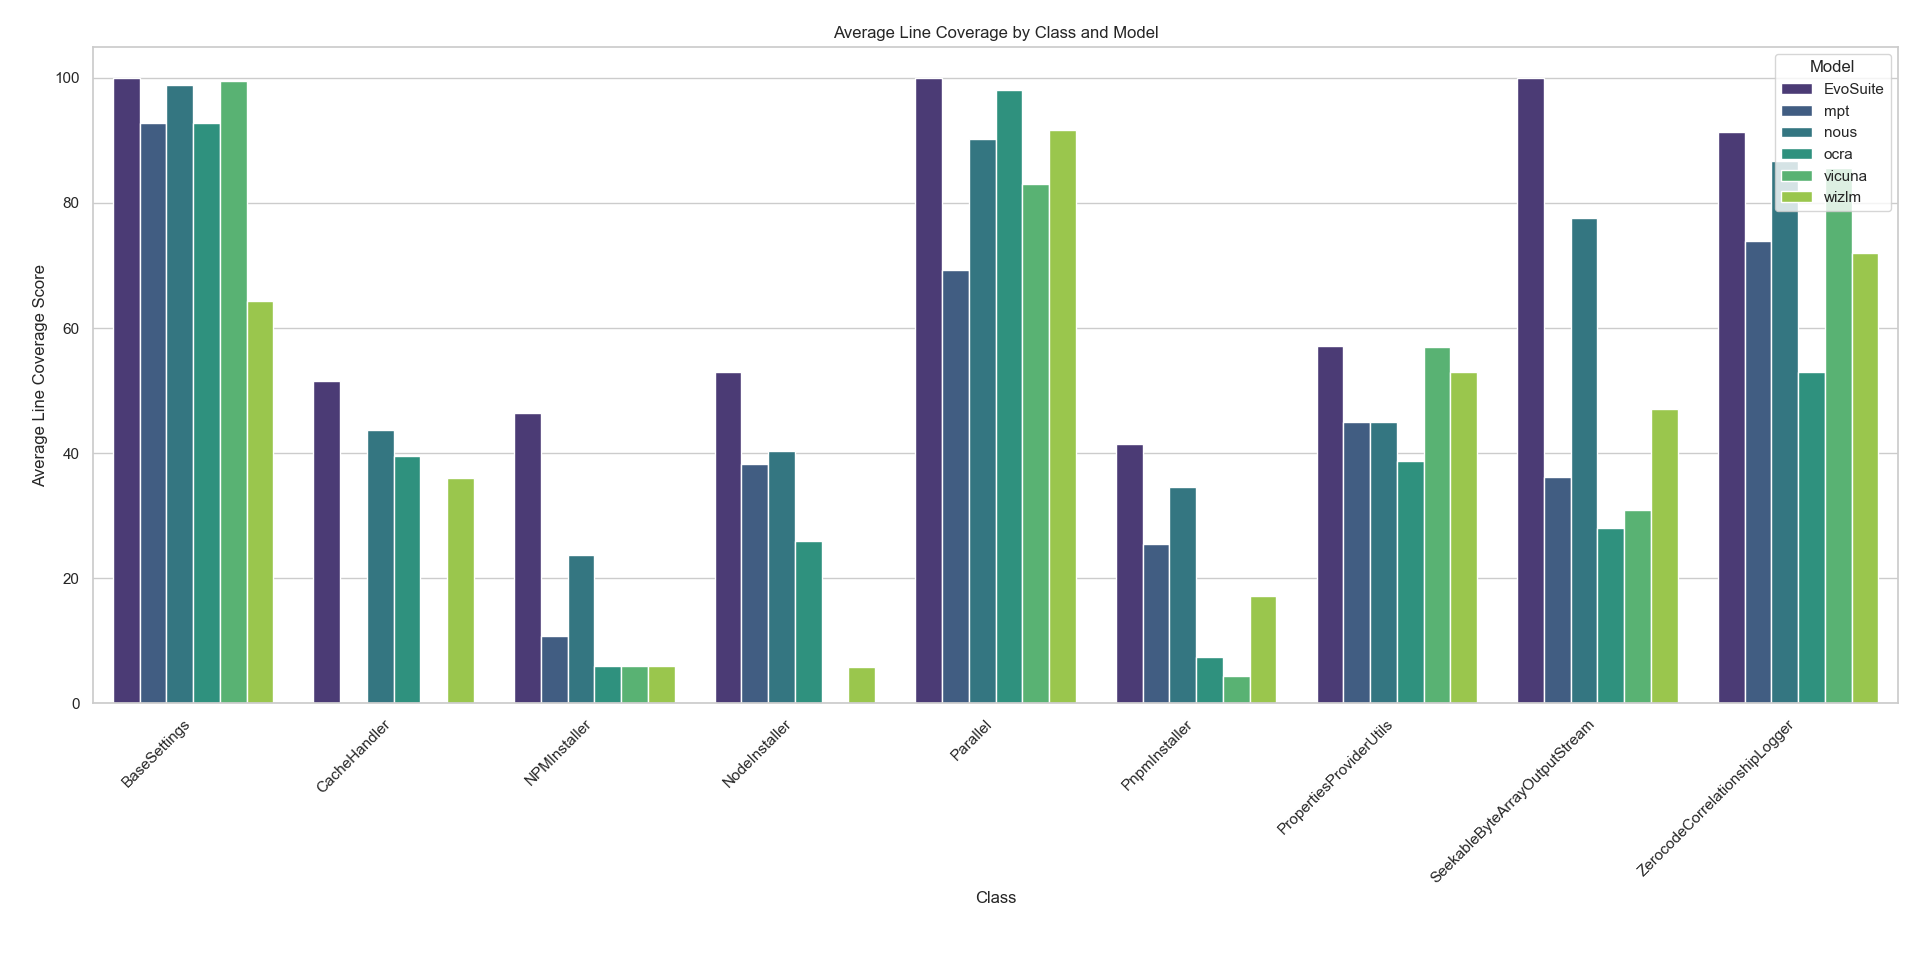
\includegraphics[width=1\textwidth]{images/line_coverage_avg.png}
\caption{Average Line Coverage by Class and Models}
\label{fig:line_coverage}
\end{figure}

\begin{figure}[H]
\centering
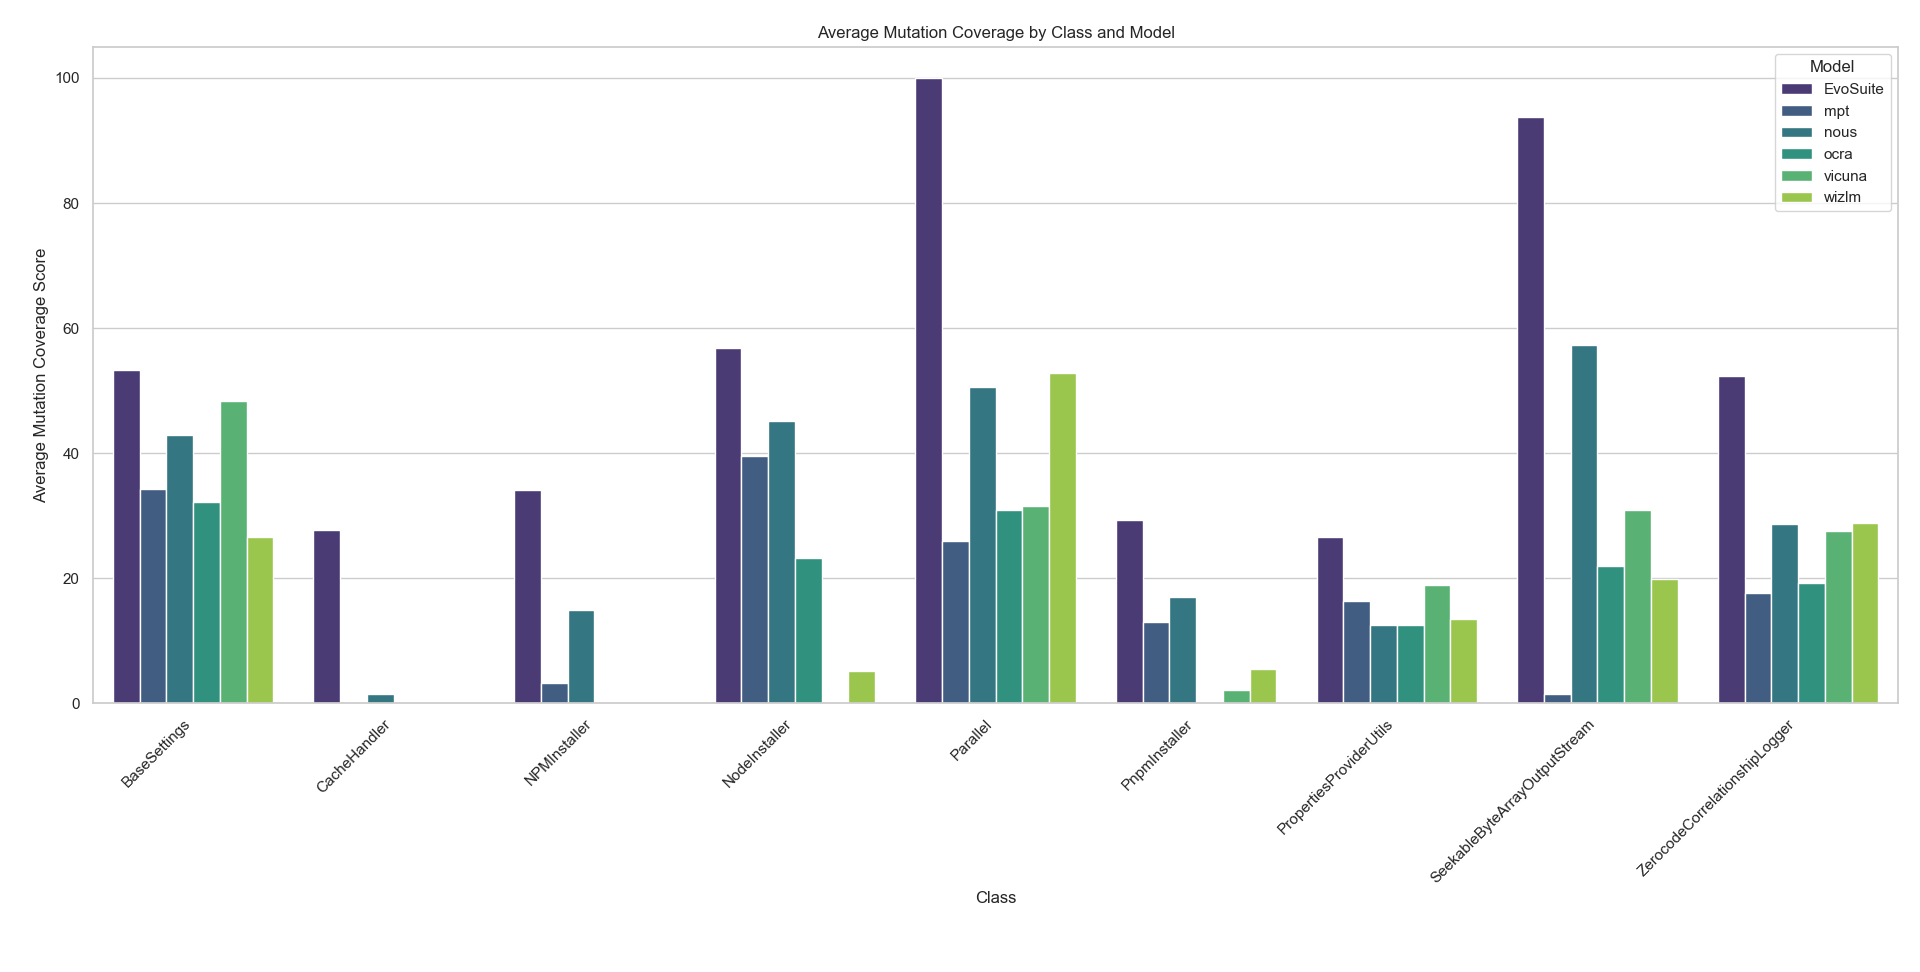
\includegraphics[width=1\textwidth]{images/mutation_coverage_avg.png}
\caption{Average Mutation Coverage by Class and Models}
\label{fig:mutation_coverage}
\end{figure}

\begin{figure}[H]
\centering
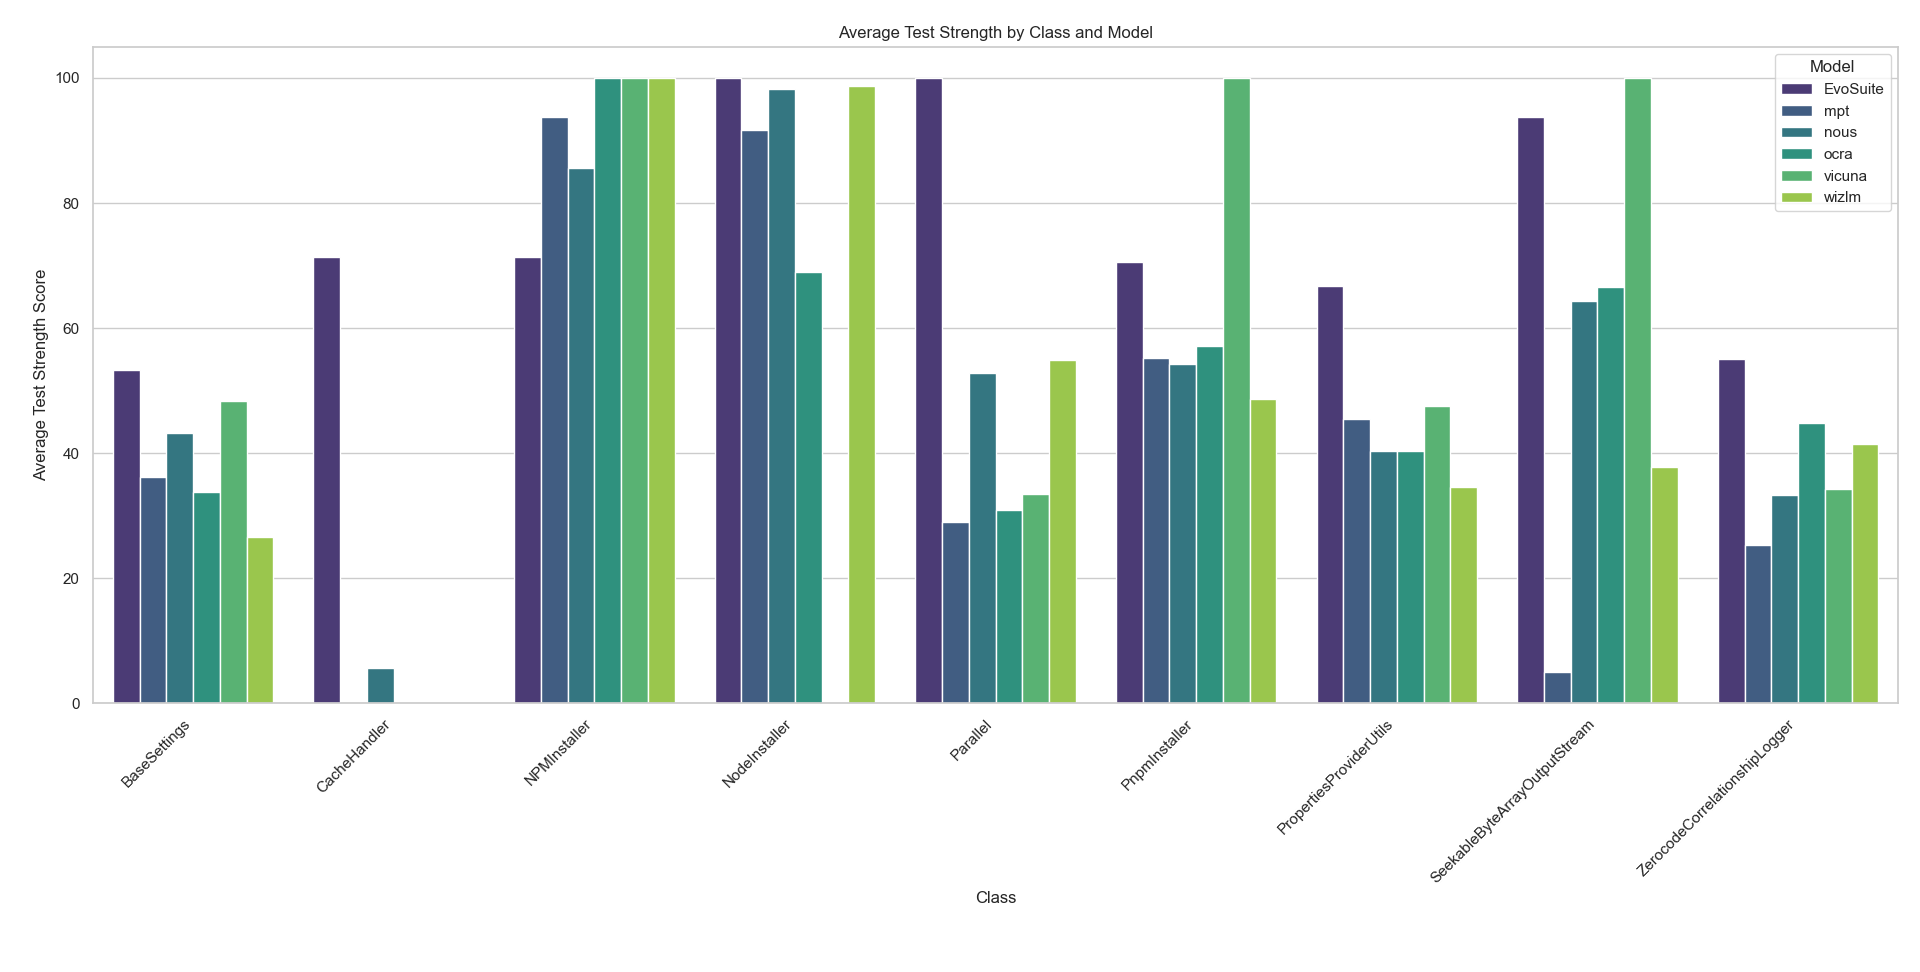
\includegraphics[width=1\textwidth]{images/test_strength_avg.png}
\caption{Average Test Strength by Class and Models}
\label{fig:test_strength}
\end{figure}

\begin{figure}[H]
\centering
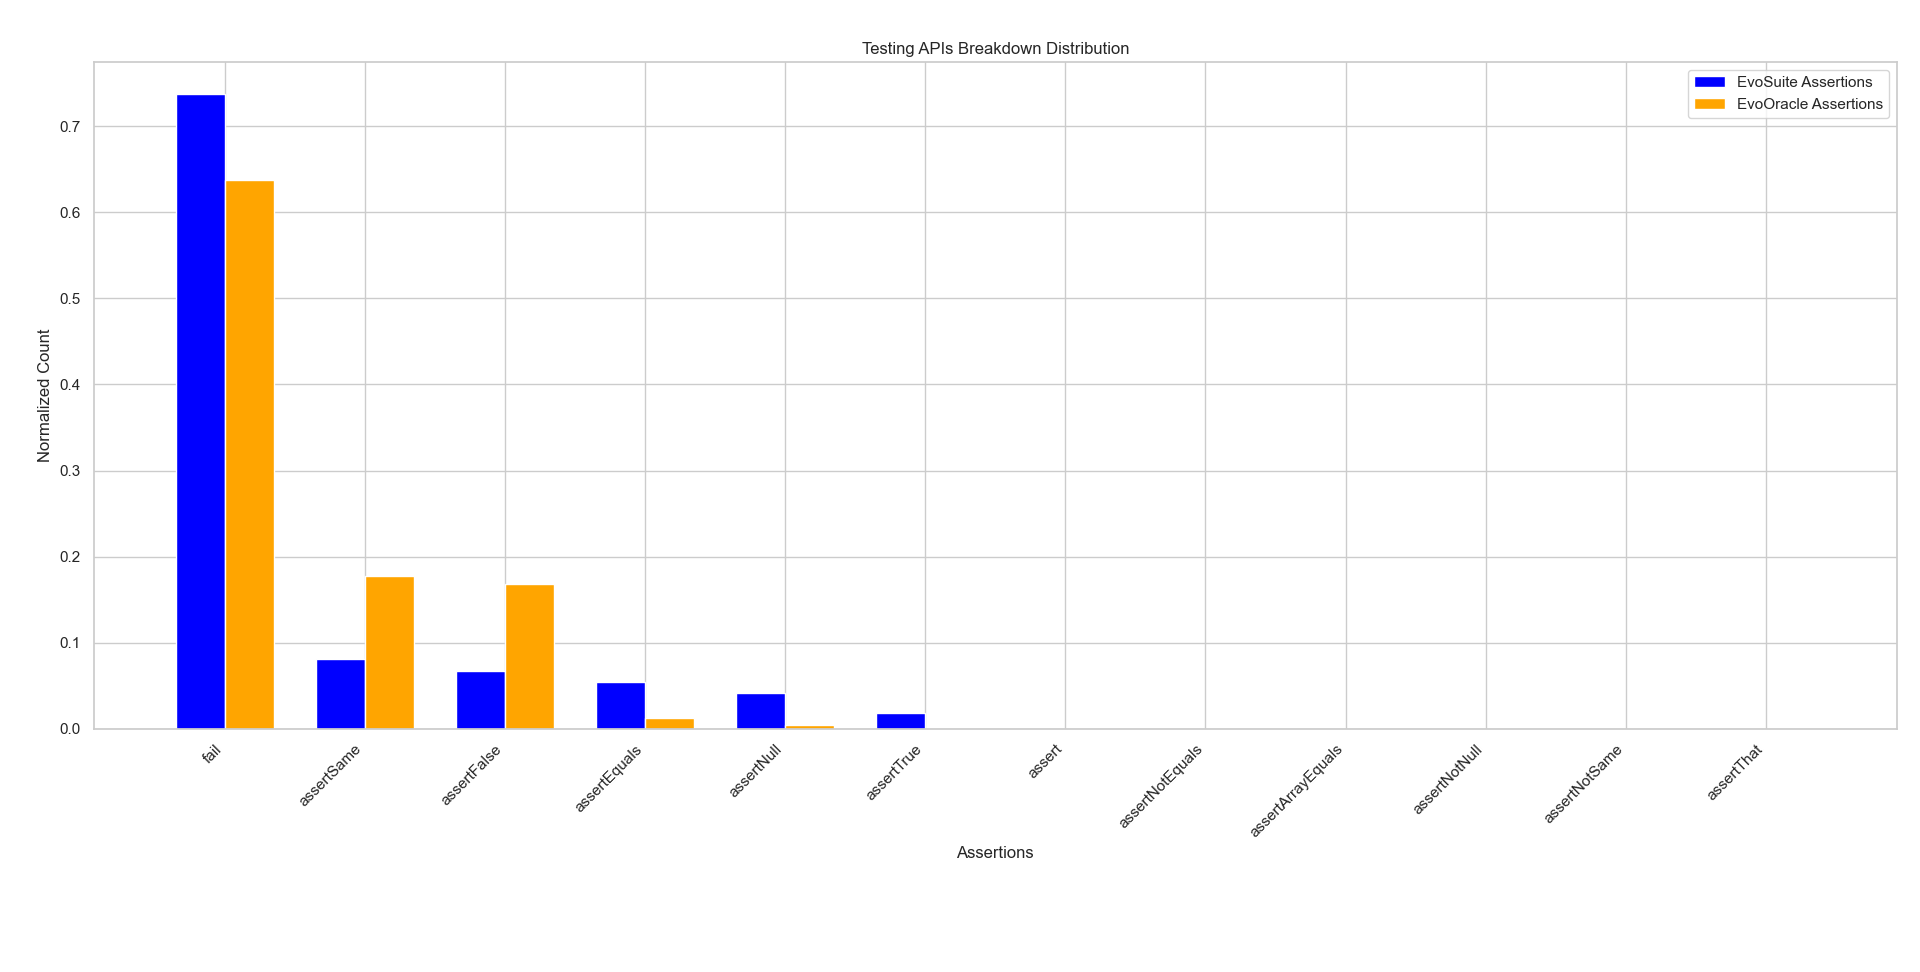
\includegraphics[width=1\textwidth]{images/test_api_distribution.png}
\caption{Testing APIs Breakdown Distribution: EvoSuite vs EvoOracle}
\label{fig:test_api_distribution}
\end{figure}

\begin{figure}[H]
\centering
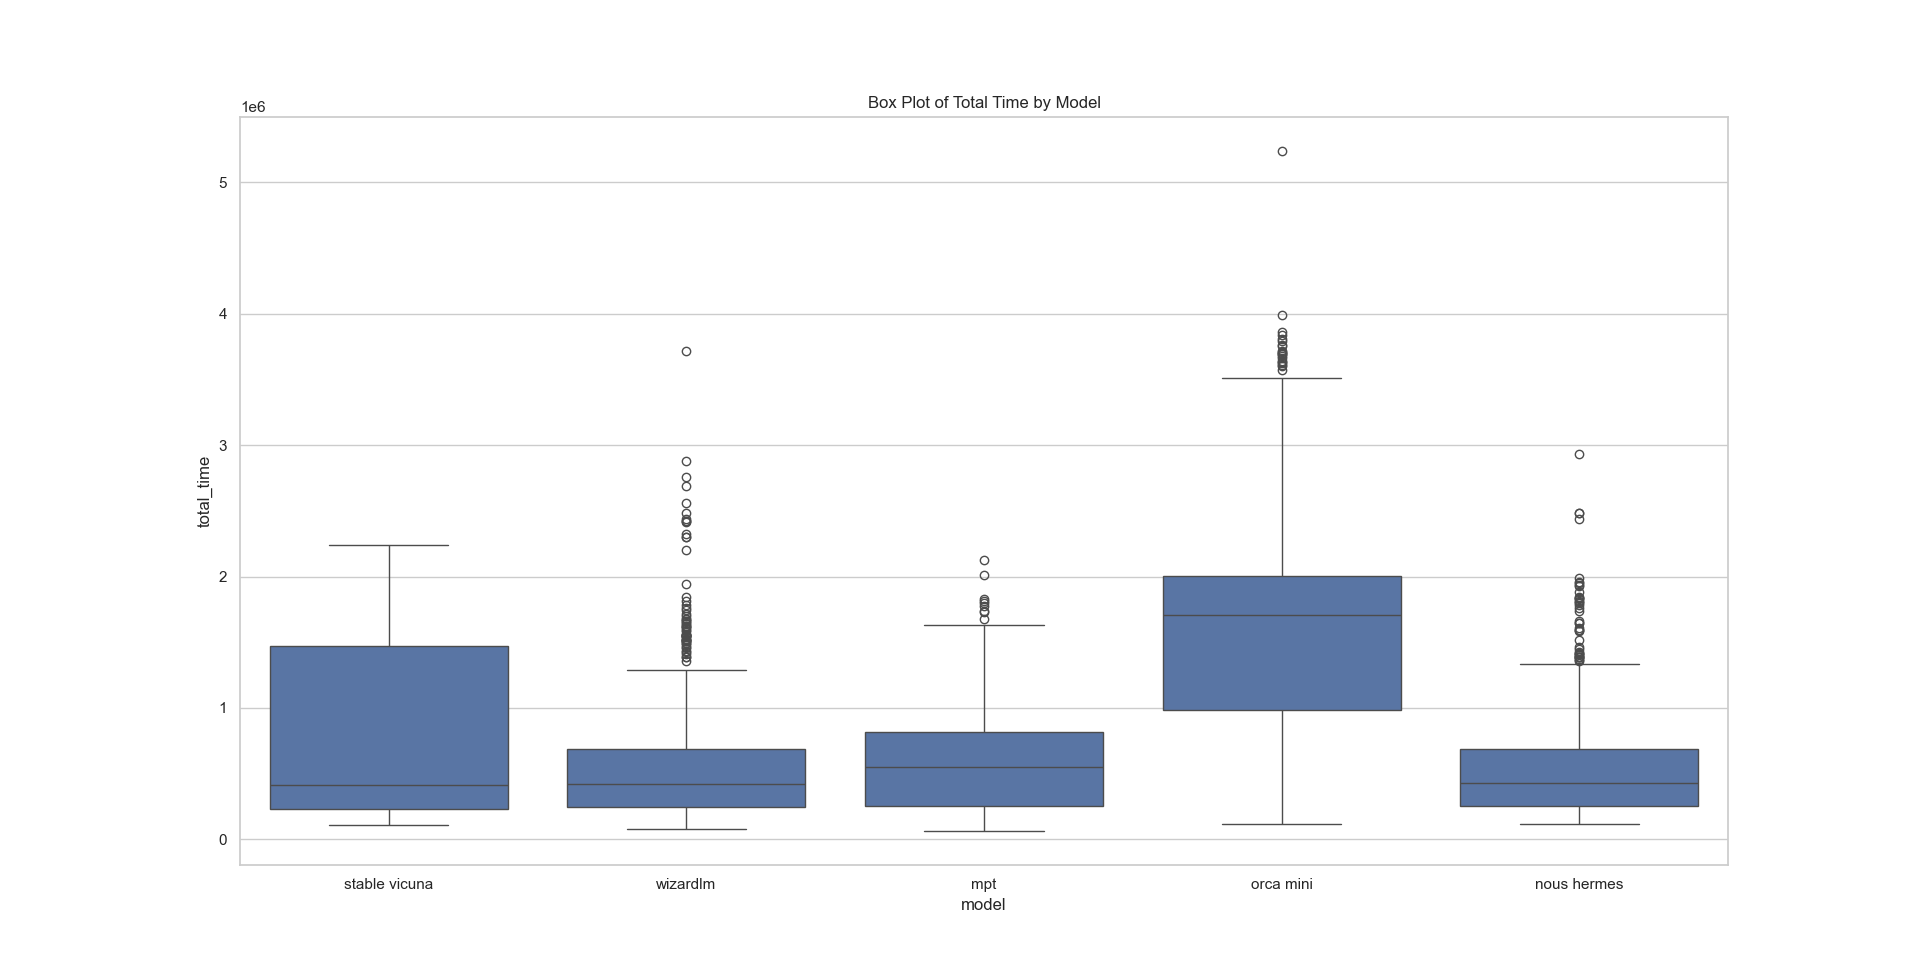
\includegraphics[width=1\textwidth]{images/time_by_model.png}
\caption{Total time taken by Models}
\label{fig:time_models}
\end{figure}

\begin{figure}[H]
\centering
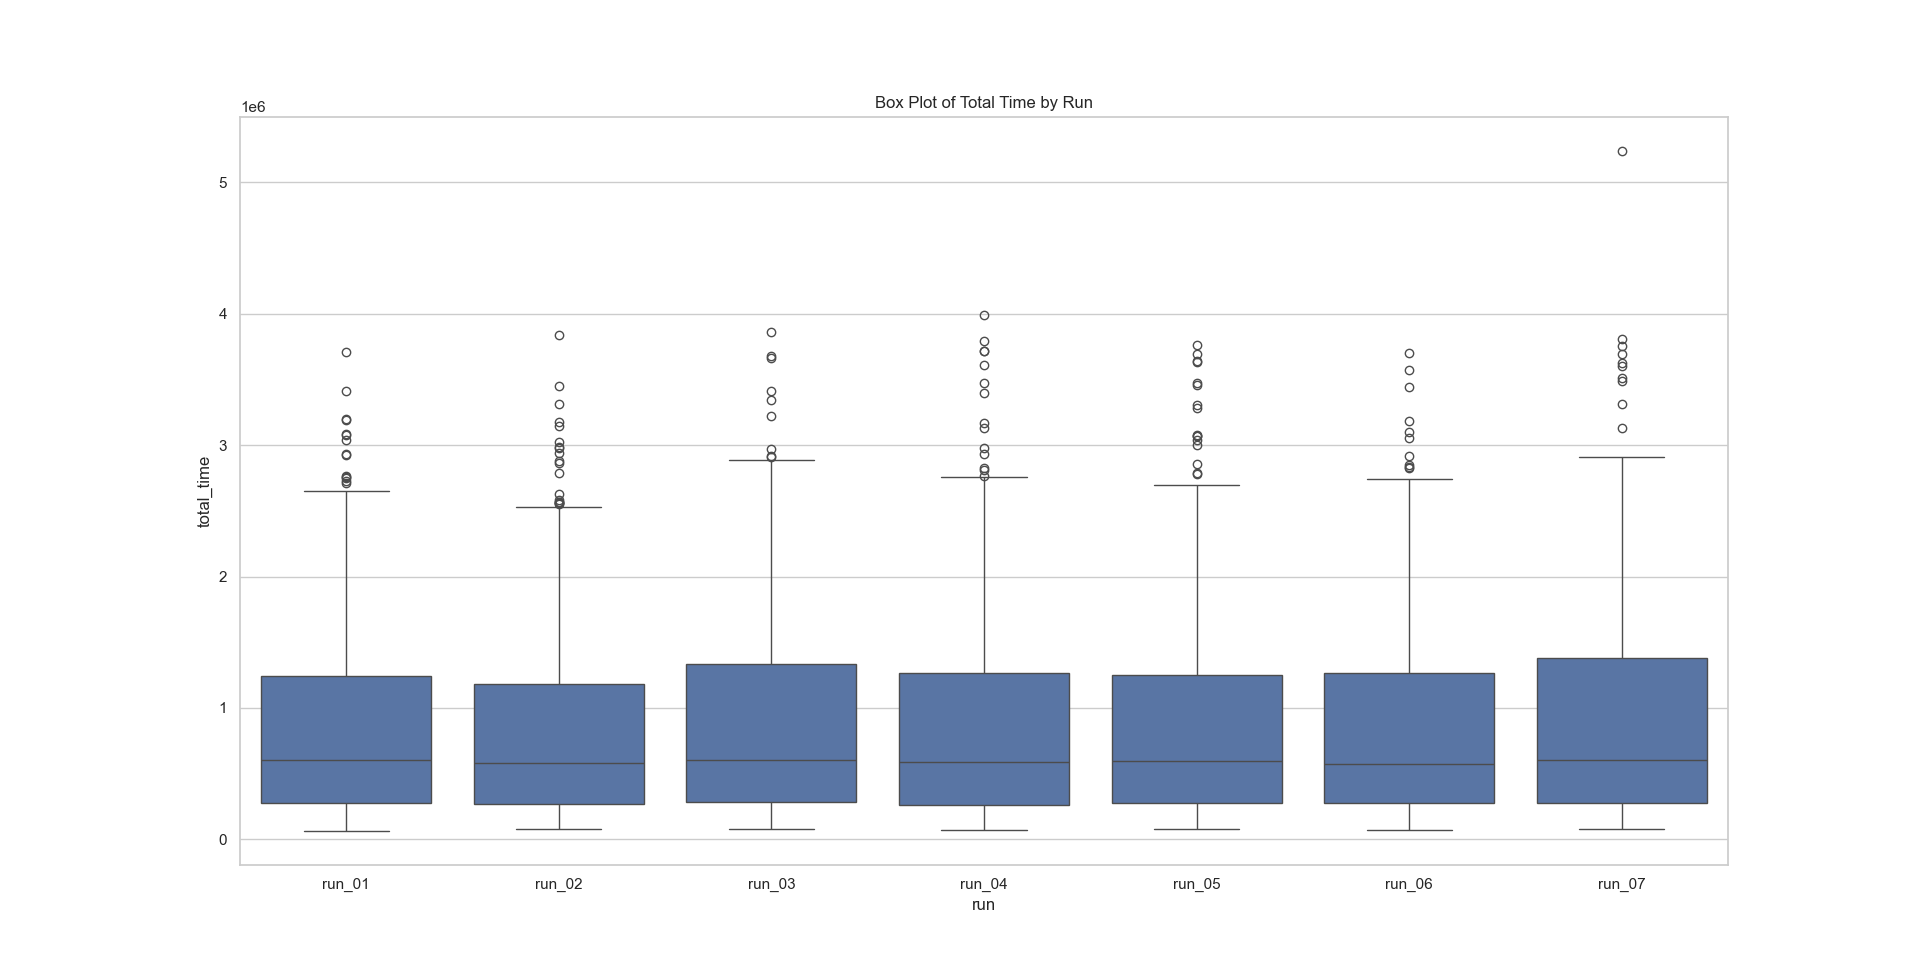
\includegraphics[width=1\textwidth]{images/time_by_runs.png}
\caption{Total time taken by each run}
\label{fig:time_runs}
\end{figure}

\begin{figure}[H]
\centering
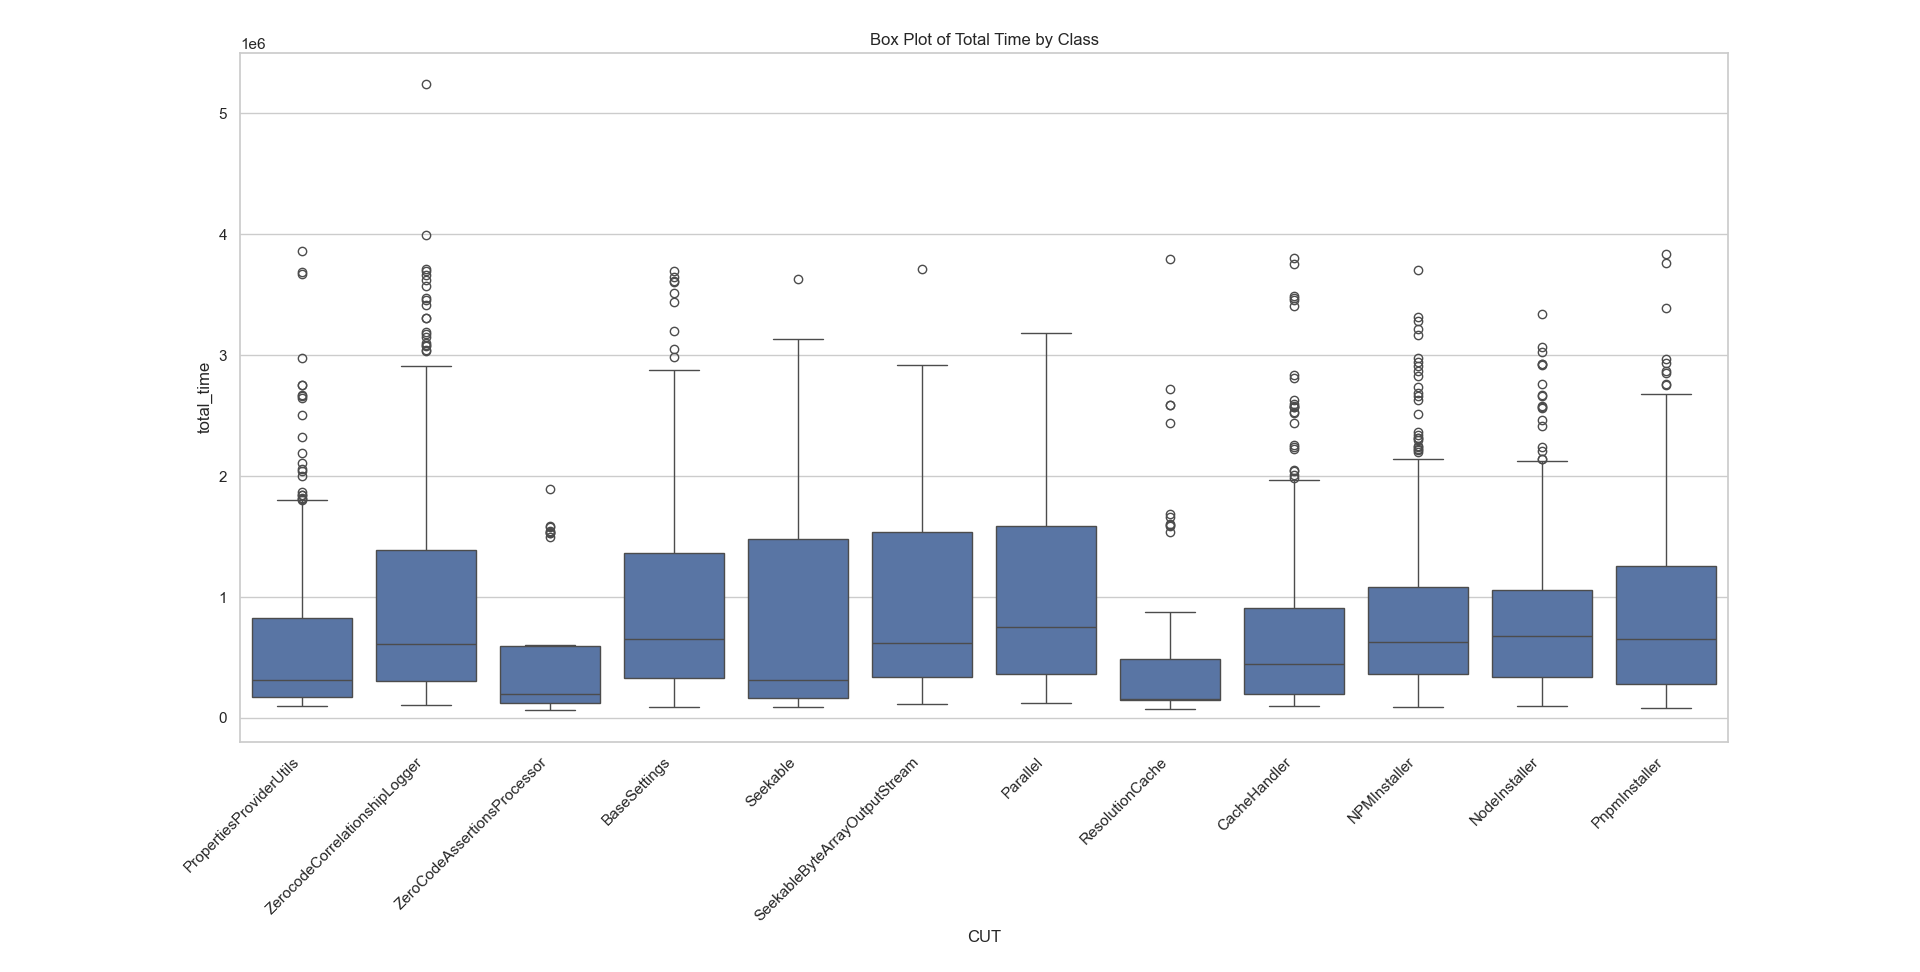
\includegraphics[width=1\textwidth]{images/total_time_by_class.png}
\caption{Total time taken by each class}
\label{fig:time_class}
\end{figure}

\begin{figure}[H]
\centering
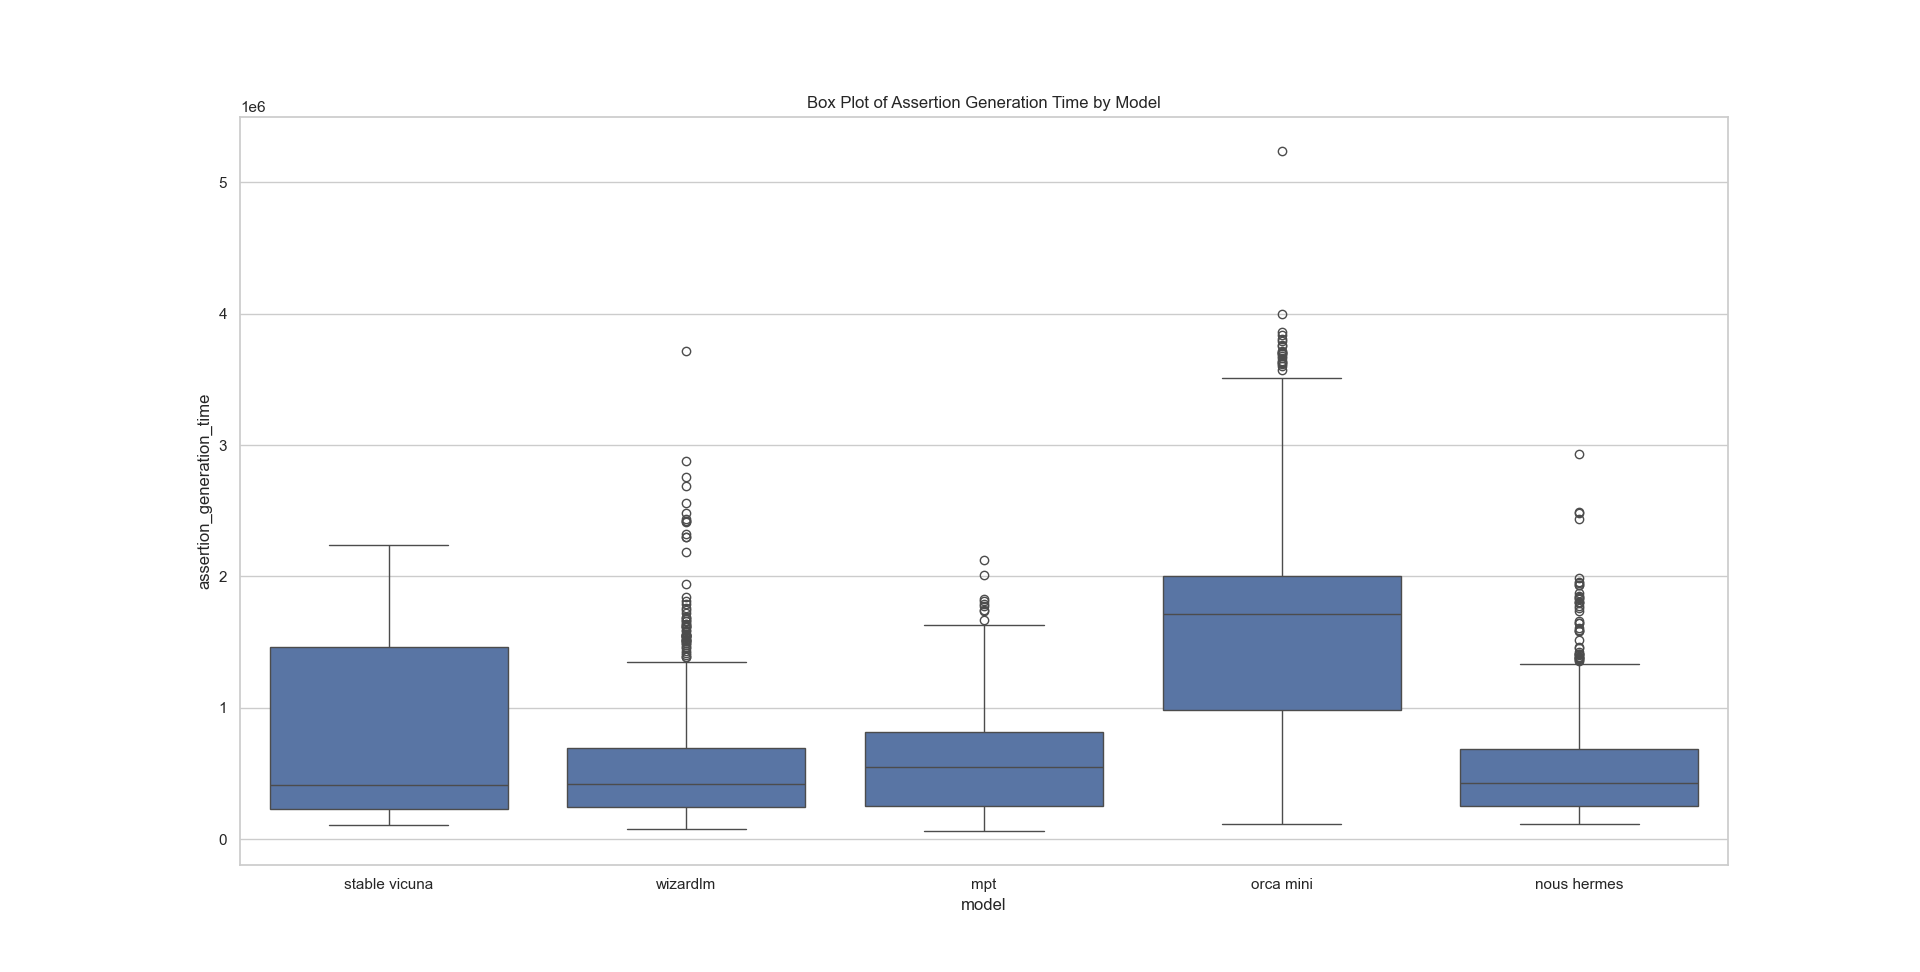
\includegraphics[width=1\textwidth]{images/assertion_time_by_model.png}
\caption{Assertion generation time taken by each model}
\label{fig:assertion_time_models}
\end{figure}

\begin{figure}[H]
\centering
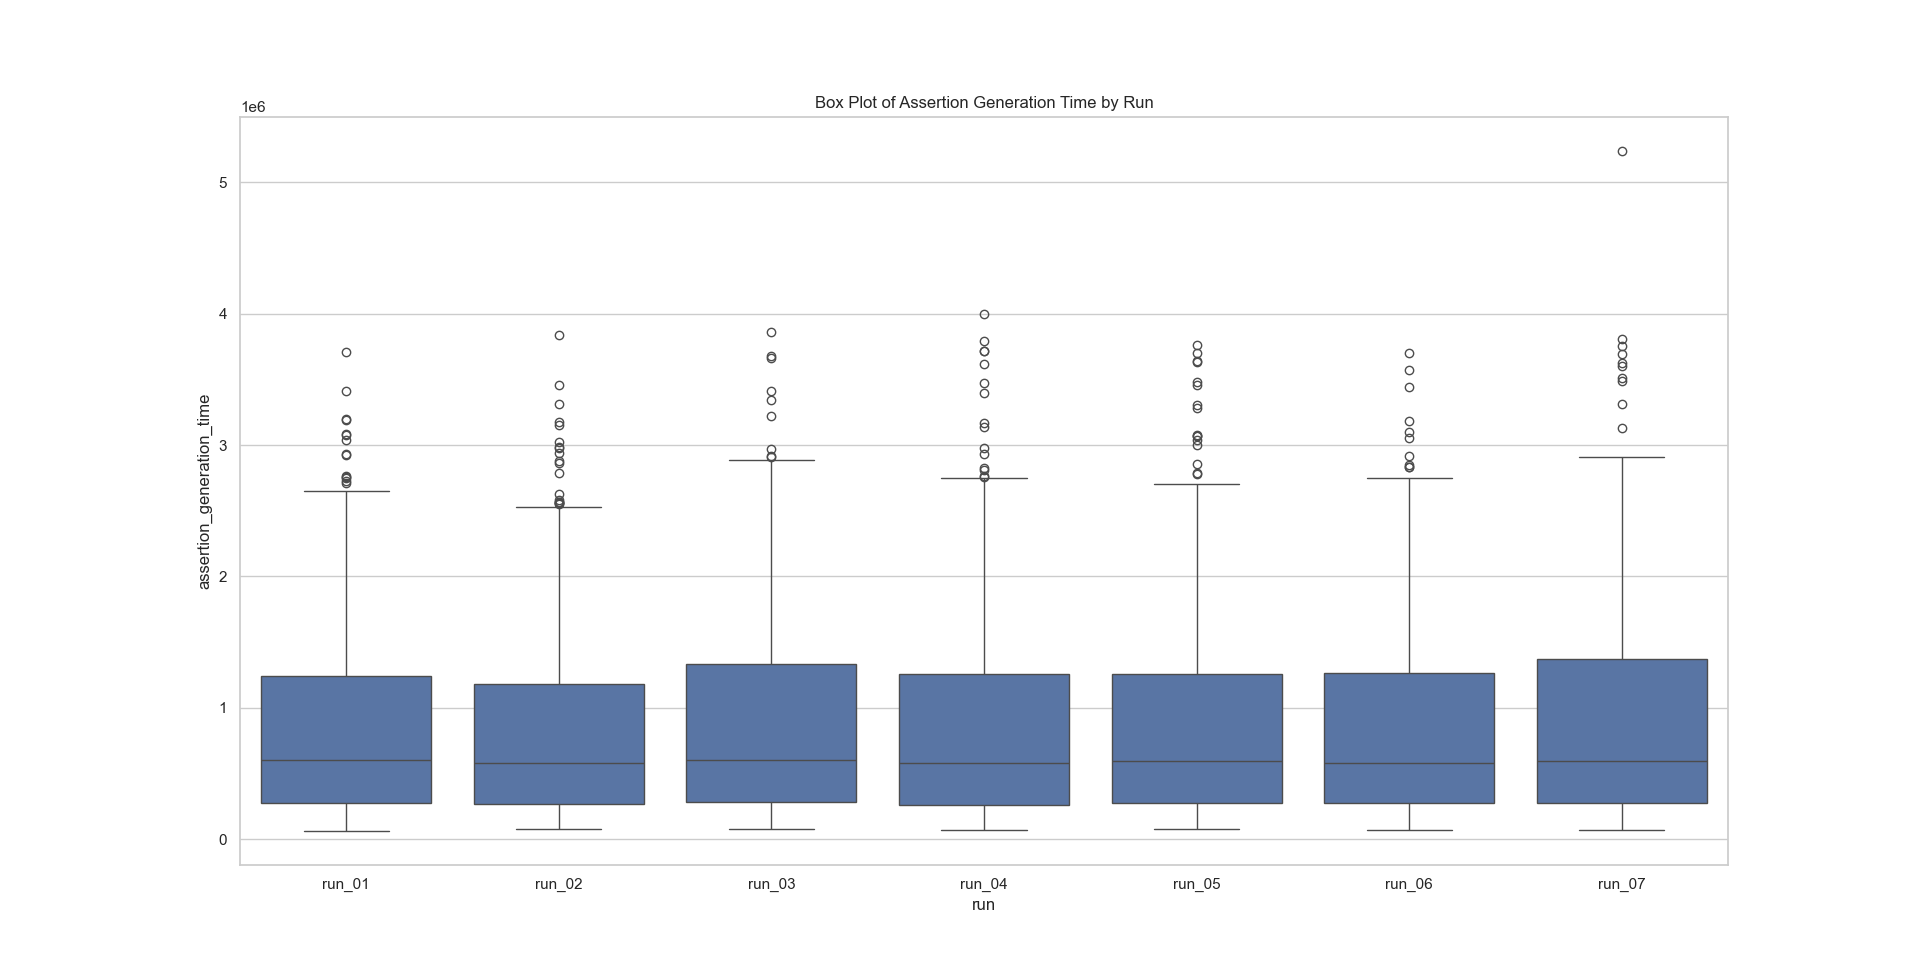
\includegraphics[width=1\textwidth]{images/assertion_time_by_runs.png}
\caption{Assertion generation time taken by each run}
\label{fig:assertion_time_runs}
\end{figure}

\begin{figure}[H]
\centering
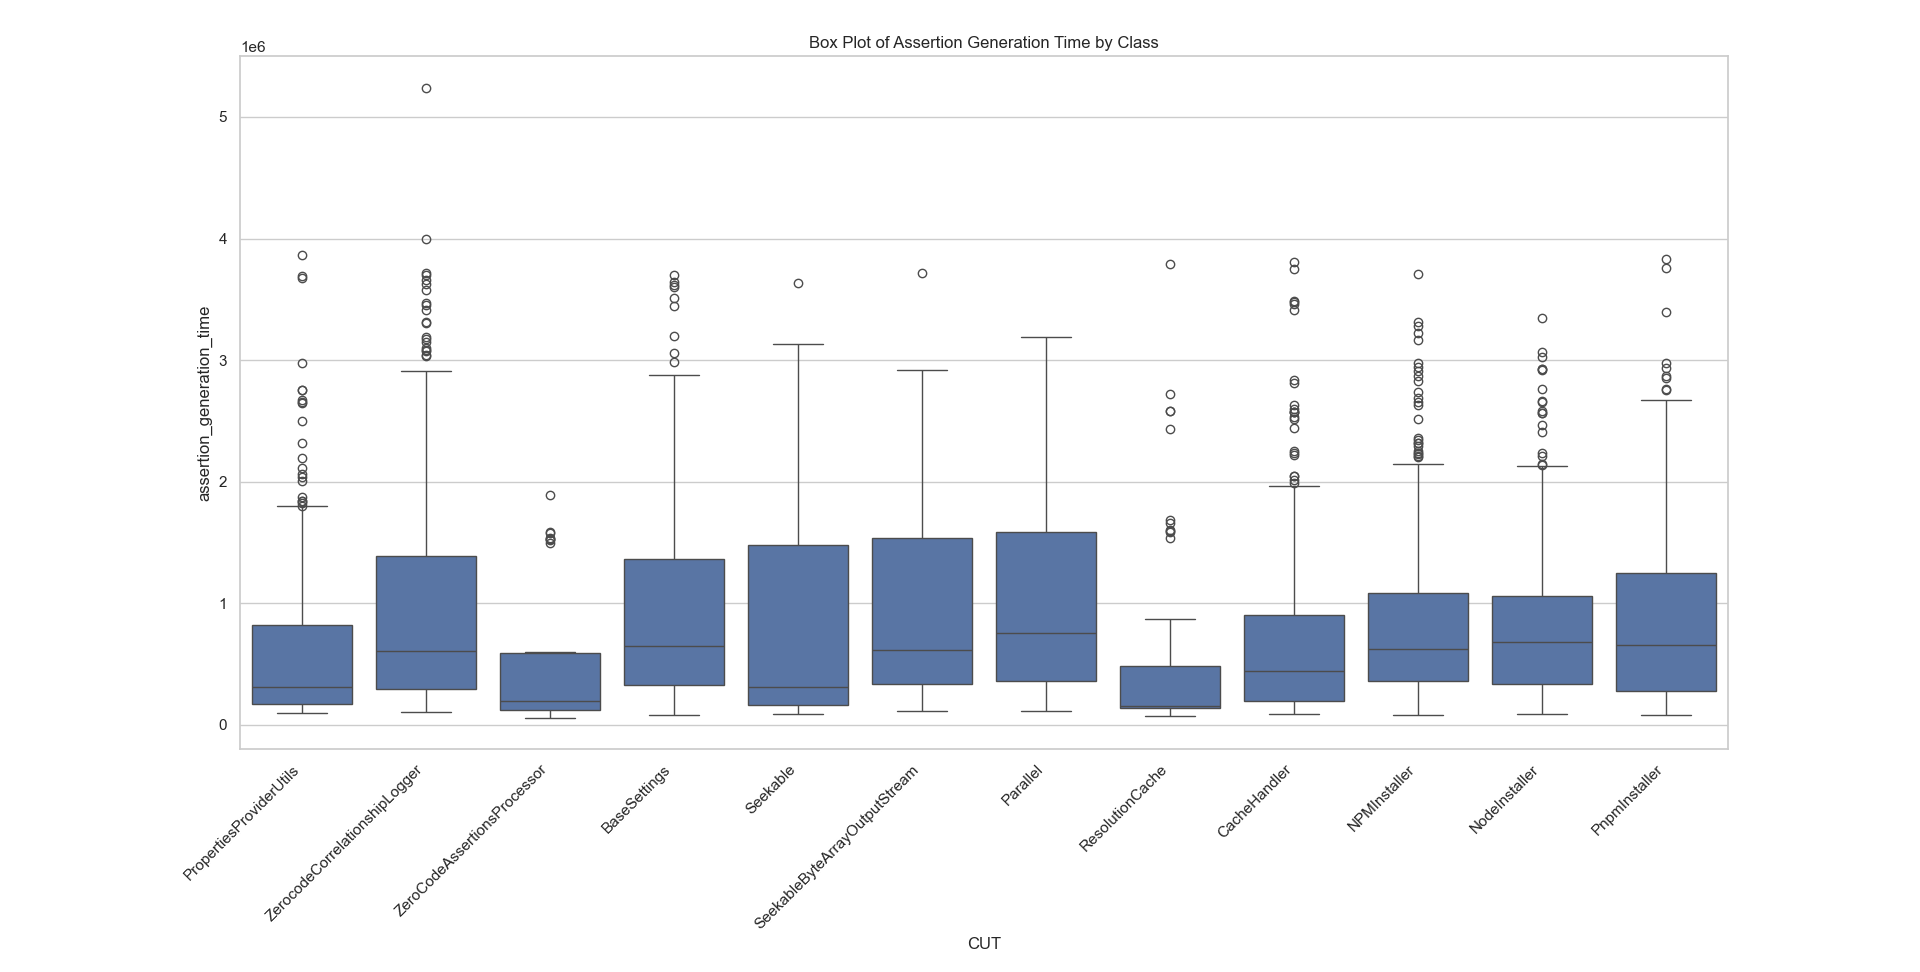
\includegraphics[width=1\textwidth]{images/assertion_time_by_class.png}
\caption{Assertion generation time taken by each class}
\label{fig:assertion_time_class}
\end{figure}

\vspace{0.1 cm}
\subsection{RQ2}
\label{sec:results_rq2}
\vspace{0.1 cm}

In this subsection, an overview of ...

\section{Threats to Validity}
\label{sec:t2v}
\vspace{0.2 cm}

The study acknowledges several potential threats to its validity.

\begin{enumerate}
    \item \textbf{Randomness in LLM Outputs:} One significant threat to the study's validity stems from the inherent randomness associated with Large Language Models (LLMs). The generated outputs are subject to variations based on the model's training conditions and prompt inputs, potentially impacting the reproducibility and consistency of results. In order to minimize the variation, we ran each experiments 7 times and took the median results.

    \item \textbf{Generalizability to Diverse Datasets:} The study recognizes the potential limitation of generalizability to other datasets or programming languages. The findings, rooted in the analysis of Java projects from GitHub, may not extend seamlessly to different programming communities or languages, highlighting a domain-specific consideration.

    \item \textbf{Dataset-Induced Bias:} The dataset itself, composed of Java projects sourced from GitHub, introduces a possible bias reflective of the practices and characteristics specific to the Java programming community on this platform. This inherent bias could influence the study's conclusions and their applicability to broader software development contexts.

    \item \textbf{Concerns of Data Leakage:} In addressing concerns related to data leakage, the study takes precautionary measures by excluding candidate repositories that might appear in the pretraining corpus of the LLMs. This step aims to ensure the integrity of the evaluation process and prevent inadvertent leakage of information.

    \item \textbf{Selection Bias from Compilation and Execution Requirements:} The imposition of specific compilation and execution requirements, such as using Maven as the package manager and ensuring compatibility, introduces a potential source of selection bias. The study acknowledges the impact of these criteria on the composition of the chosen repositories, potentially affecting the representativeness of the dataset.

    \item \textbf{Evaluation Metrics Limitations:} The study recognizes the limitations of the chosen evaluation metrics and criteria. While these metrics provide a quantitative basis for assessment, they may not comprehensively capture the nuanced aspects of LLM-based test oracle generation. This acknowledgment indicates a need for a holistic understanding beyond the quantitative measures employed.
\end{enumerate}

These considerations collectively contribute to the study's robustness and transparency, providing insights into potential factors that may influence the interpretation and application of its findings.

\section{Discussion}
\label{sec:discussion}
\vspace{0.2 cm}

Diving into a comprehensive discussion of our experiments and findings unveils nuanced insights into the intricate landscape of automated testing practices, particularly in the context of leveraging Large Language Models (LLMs) for test oracle generation. The empirical analysis of our approach to generating oracles for unit test cases provides a nuanced understanding of the challenges and potential breakthroughs in this domain. As we navigate the landscape of automated testing, it becomes evident that the multifaceted nature of test cases poses unique challenges that demand innovative solutions.

The comparative analysis between LLM-generated assertions and traditional automated test generation tools, exemplified by EvoSuite, brings to light unexpected and valuable results. The effectiveness and efficiency of LLM-based approaches did not universally outperform traditional methods, marking a noteworthy observation that prompts a deeper exploration into the factors influencing assertion quality and the overall testing workflow.

Surprisingly, LLMs, despite their profound capabilities in understanding natural language, grapple with the complexity of translating this understanding into precise code-related tasks. This observation raises critical questions about the adaptability of LLMs to the diverse nature of test cases, each with its unique intricacies and requirements for meaningful assertions. As developers interact with LLM-generated assertions, a spectrum of sentiments emerges, reflecting the potential and challenges in incorporating advanced language models into the day-to-day software development processes.

Moreover, the results of Research Question 2, indicating an average time of 8.24 minutes for assertion generation for a single test case, shed light on a usability challenge. This prompts considerations about real-world practicality, prompting us to explore alternative approaches, including leveraging APIs like ChatGPT for faster and potentially more efficient interactions.

\section{Future Work}
\label{sec:discussion}
\vspace{0.2 cm}

The journey of our research extends beyond the current findings, venturing into unexplored territories of innovation and improvement. An essential area of exploration lies in the improvement of the assertion generation process. As we aim to enhance the usability and adoption of LLM-generated assertions, integrating them seamlessly into continuous testing pipelines emerges as a promising avenue. However, this involves overcoming challenges related to scalability, parallelization, and real-time responsiveness, aligning with the dynamic nature of agile development practices.

In our quest for more effective assertion generation, the prospect of fine-tuning LLMs specifically for software testing contexts captures attention. Tailoring models to recognize and generate assertions in alignment with testing requirements may hold the key to enhancing precision and relevance. Addressing the limitations observed in this study requires dedicated efforts in model refinement, with a focus on developing specialized training strategies that align LLMs more closely with the intricacies of code-related tasks.

Furthermore, the potential integration of LLM-generated assertions into developers' daily workflows calls for a holistic approach. This involves developing more intuitive interfaces, visualizations, and feedback mechanisms that facilitate seamless collaboration between developers and LLMs. User-friendly integration is paramount, requiring a delicate balance between advanced technologies and practical usability.

As we look towards the future, investigating adaptive strategies for dynamically adjusting LLM configurations during the assertion generation process stands out as a crucial research direction. This entails leveraging machine learning techniques to optimize settings based on evolving testing needs, providing a dynamic and responsive framework for assertion generation.

Another dimension of exploration involves delving into methodologies for incorporating developer intent and context explicitly into the assertion generation process. Interactive prompts or mechanisms that empower developers to guide LLMs in generating assertions aligned with their testing goals present an exciting avenue for enhancing the relevance and applicability of generated assertions.

Conducting in-depth user studies to assess the long-term usability and acceptance of LLM-generated assertions in real-world development scenarios becomes imperative. Understanding how developers seamlessly incorporate LLM-generated assertions into their routine testing practices offers valuable insights into the practical implications of our research.

To broaden the impact and relevance of our approach, extending language and framework support for LLM-based assertion generation to encompass a broader spectrum of programming languages and testing frameworks becomes a priority. This ensures that the benefits and insights derived from our research can be applied across diverse software development ecosystems.

In conclusion, our journey into the realms of automated testing with LLMs serves as a foundation for continuous exploration and innovation. The dynamic intersection of artificial intelligence and software engineering presents boundless opportunities for reshaping the landscape of testing practices, and our ongoing commitment is to contribute meaningfully to this evolving narrative.